\chapter{HOUSING}
\begin{chapquote}{Peter Todd}
``You can never really know if something is secure. You only know when it’s been exploited and no longer secure.''
\end{chapquote}

\section{Home equity and personal balance sheets}\label{home_equity}

An asset is something that is going to give you some economic benefit. A liability is an economic obligation to someone else. The equity is the difference between assets and liabilities.
Assume I have \$250k in cash, no assets, no liabilities. Then, I borrow \$750k from the bank to buy a \$1m house. My equity is still \$250k, but if my house, for some unforeseen reason, depreciates to 800k, then my equity will decrease. In this case, a drop of 20\% of my assets corresponds to a drop of 80\% of my equity.
Instead, in a more optimistic scenario, my house appreciates to \$1.2m, hence +20\%, my equity becomes \$450k, hence +80\%, a make-believe amount of wealth. 
In the second situation, I can go back to the bank and show them that now I have \$450k in equity, but I want cash instead. They agree to give me money, but up to 75\% of the value of my house: \$900k. Subtracting what I owe the bank, I get \$150k in cash. This money come from the equity of my house basically. Now I have \$1.2m (house) + \$150k (cash) of assets and \$750k (house loan) + \$150k (equity loan) of liabilities for a total equity of \$450k, unchanged. What I can do now, though, is to go on vacation and spend all my cash. When I come back from vacation, I'll have \$300k in equity. I was able to do this because I borrowed money against the value of my house.

\section{Mortgages} \label{mortgages}
Assume I want to buy a house but I only have 25\% of the money needed to buy it, which is \$500k. I can ask the bank for a loan for the other 75\%. The bank will give me the loan, but the home title goes to the bank to secure the loan. While I pay back my loan, I live in the house, but the bank owns it as a security. This pledging of the title is a mortgage (pledge: that will die when I pay back my loan).

Let's assume there is a 5.5\% fixed annual interest rate and it is a 30-year loan. The monthly interest rate is 0.46\% and the monthly payment is roughly \$2130. Let's analyze the table in Figure \ref{fig:mortgage_xlsx}, starting from the first line. 

\begin{figure}[h!]
\centering
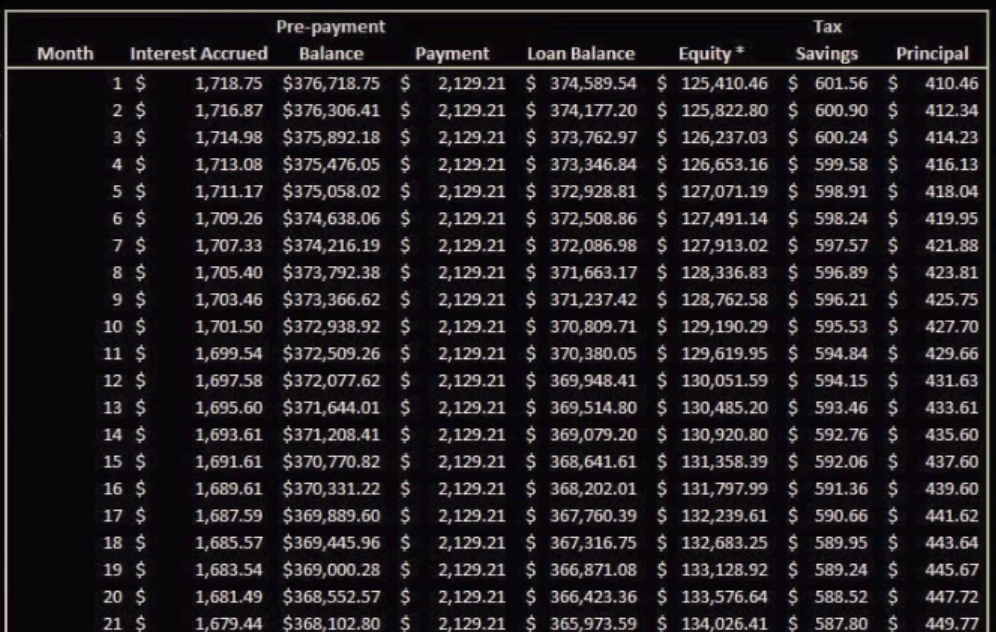
\includegraphics[width=0.8\textwidth]{images/mortgage_xlsx.png}
\caption{Mortgage spreadsheet}
\label{fig:mortgage_xlsx}
\end{figure}

The second column is obtained by multiplying \$350k by the monthly interest rate. The third column is my total debt I have with the bank which is the sum of my loan plus the interest accrued. The fourth column is simply the monthly payment. The fifth column is the total debt after the monthly payment. The sixth column is my equity, which was initially \$125k. The increment in its value is coming from the difference between my monthly payment and the monthly interest (fourth minus second column). The second line is similar, but the second column is obtained by multiplying the monthly interest rate by the fifth column of the previous row. The procedure is the same, but now I pay less interest as the loan is lower. My monthly payment is fixed, but with time there is less interest to pay and more money goes into the payment of the loan. The money paid in interest is deductible from taxes, which means I can subtract it from my income and pay less taxes. To compute the tax savings, one can simply multiply the interest accrued by the tax rate. 

\subsection{Adjustable rate mortgages}
So far, the interest rate was considered to be fixed. Sometimes, though, it is not fixed, like in the case of 5/1 ARM. This is a hybrid adjustable rate mortgage, where during the first 5 years there is a fixed rate, then it is adjustable every year―it usually lasts 15-30 years. The bank can change the rate according to some index (e.g., 10-year treasury bonds) and this is obviously riskier (interest rate risk). In the case of fixed interest rate is the lender at risk, in the case of adjustable interest rate is the borrower at risk.
\subsection{Balloon payments}
A different scenario is the "balloon payment". Here, the bank borrows money and sets a fixed interest rate for a 30-year loan, but it lasts only 10 years, which means after 10 years of fixed interest rate, the borrower has to pay back the remaining loan. This might seem a bit illogical, but it's not. In the 10 years, the borrower has less risk as the interest rate is fixed, and after that, the bank has no risk at all (this may lead the bank to offer a lower fixed interest rate). Also, the borrower might decode for this kind of payment if he plans to sell the house or take another loan if some cash is suddenly available (inheritance, for example).

\subsection{A bad situation}
Let's say you want to buy another house at \$200k, but you only have \$50k. Again you ask for a loan to the bank and you get \$150k. Unfortunately you lose your job and you can't pay the loan anymore and in addition the house has lost its original value and you're able to sell it for \$120k. That's not a good situation and you have two options: foreclosure, where you basically default and you're reported to credit agencies or short selling. In the latter case, you ask the bank to accept your house at \$120k and forgive you about the missing \$30k. In addition you should specify the bank not to be reported to the credit agencies, otherwise you won't be able to get another loan in many years to come. The missing \$30k though as to be considered as part of your income.

\subsection{Loan and present values}
How to compute the monthly payment seen in Figure \ref{fig:mortgage_xlsx}? Let's assume the amount of the loan is $L$, the monthly interest is $i$, $n$ is the number of months and $p$ is the monthly payment we're looking for. My first monthly payment will be:

\begin{equation}\label{eq:1monthly_payment}
p_1 = L(1+i) ;
\end{equation}

while the second would be 

\begin{equation}\label{eq:2monthly_payment}
p_2 = \bigg(L(1+i) - p_1\bigg)(1+i);
\end{equation}

and so on with the third, fourth, ..., till the n-th.
We want to pay always the same amount per month, which means: $p_1 = p_2 = ... = p_n = p$. What we also want is that after all the n payments, there is no more debt, so the loan has been covered. If we solve equation~\ref{eq:1monthly_payment} for $L$ and then again we solve equation~\ref{eq:2monthly_payment} for $L$ we would see a pattern which is the following:

\begin{equation}\label{eq:loan_sum}
L = p\sum_{j=1}^{n} \dfrac{1}{(1+i)^j};
\end{equation}

What is this? The loan can be seen as a sum of the present values of all my payments in the future (future value discounted by the interest rate). Equation~\ref{eq:loan_sum} is a geometric series and the solution is known. It turns out that $p \cong \$1200$ 

\section{Home buying process}

\subsection{Titles and insurances}
When someone is buying a house, she has to make sure that the supposed-to-be owner of the house is able to provide a document certifying that he's the real owner (possession is not always ownership). This document is called title or deed. Suppose a house is built and owned by Alice and when she dies she has absolutely no relatives to inherit the property and it is given to the city council and then sold legally to Bob. What if after 20 years, Carl shows up proving that he was the son of Alice and the house should belong to him? Bob would be in a very bad situation. To protect Bob from rare events like this, there are title insurances that will cover the costs.

\subsection{Escrow accounts}
Another critical situation arises when a buyer and a seller agree on a contract: the seller will give the title of the house to the buyer and the buyer will pay the house to the seller. But, should the buyer pay first than receiving the title or should the seller give the title before the payment? They can't trust each other, so what happens is that they need a trusted third party, an escrow agent and they open an escrow account. It will make sure that once all the money has been collected, the title is given to the buyer. After that, the escrow account is closed.
